\scanpage{451}
\mspage{228}

and we will have
\[
(23)\qquad X_g=X_{g,i}\amalg_{\partial\widetilde M}\widetilde M
\]
by a well-determined \unsure{homeomorphism} of $\partial\widetilde M$ with an open and closed subset of $\partial X_{g,i}$. Moreover, we will have a canonical continuous map
\[
(24)\qquad U_0\longrightarrow X_{g,i}
\]
which defines a homeomorphism of $X_{g,i}$ with \unsure{the|the} \deleted{\unsure{manifold}} surface \unsure{obtained|obtained} by contracting the $\underset{\inserted{\substack{\parallel\\(\partial D_j)\times\varepsilon_j}}}{\uline{\partial\Delta_j}}\subset U_0$ $(g-i+1\leq j\leq g)$ using the \unsure{projections} $\partial\Delta_j\simeq(\partial D_j)\times\varepsilon_j\longrightarrow D_j$.

On the other hand, each $\widetilde M_j$ $(1\leq j\leq g-i)$, the covering \inserted{of the} orientations of the Möbius band, is isomorphic to the cylinder $S^1\times I$, and its canonical anti-involution \deleted{is identified} has no fixed point, and is identified with:
\[
(z,t)\longrightarrow(\unsure{-z}^{\deleted{\illegible{1}}},-t)
\]
(where $S^1$ is identified with the complex numbers of modulus $1$, and $I:[-1;+1]$).

Moreover, $X_0$ \inserted{\unsure{oriented|oriented},} with \unsure{its} anti-involution of the \unsure{cover\textsuperscript{ing}|covering} of $Y_0$ is identified with the ordinary sphere \deleted{\unsure{of the}}\inserted{, in a Euclidean vector space of dimension $3$}, with the anti-involution $x\longmapsto-x$.

\scanpage{452}

In summary:

\uline{Proposition} We can obtain (for $0\leq i\leq g$ fixed) the pairs $(X_g,\sigma_i)$, up to \unsure{homeomorphisms}, by taking the \deleted{\unsure{oriented}} \inserted{oriented Euclidean} sphere $X_0$, with its standard antipodism $\tau$, by taking a set of $2g$ disks \inserted{$\unsure{D'_j}\ (j\in J)$} mutually disjoint, stable under $\tau$, and a subset $I'\subset J/\tau=I$ ($I$ of cardinality $g$) with $\operatorname{card}I'=i$, \margin{introduce it later} and by \unsure{proceeding} as follows: for every $j\in I$, let $\Delta_j=D'_j\cup D''_j$ be the \inserted{union of the two} corresponding disks, and $S_j=\partial\Delta_j/\tau$, so that $S_j$ is a circle, let \figure{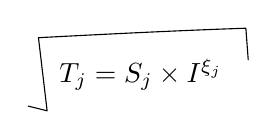
\begin{tikzpicture}[baseline=(lmfixtwentyfour.base),line cap=round,line join=round]
\node[inner sep=2.5pt] (lmfixtwentyfour) {$T_j=S_j\times\unsure{\mathbb I}^{\unsure{\xi_j}}$};
\draw[line width=.4pt]
([xshift=-3mm,yshift=-1mm]lmfixtwentyfour.south west)
-- ([xshift=-.6mm,yshift=-1.6mm]lmfixtwentyfour.south west)
-- ([xshift=-1.7mm,yshift=1.8mm]lmfixtwentyfour.north west)
.. controls ([xshift=6mm,yshift=2.2mm]lmfixtwentyfour.north west) and ([xshift=-7mm,yshift=2.7mm]lmfixtwentyfour.north east) ..
([xshift=2mm,yshift=3mm]lmfixtwentyfour.north east)
-- ([xshift=2.3mm,yshift=-1mm]lmfixtwentyfour.north east);
\end{tikzpicture}} (where $\unsure{\mathbf I|\mathbb I}=[-1,+1]$), $\varepsilon_j=\{j'\in\unsure{J|\mathbf I}\mid j'\text{ over }i\}$\inserted{$\simeq$ set of \uline{orientations} of $S_j$}, $\unsure{\mathbf I^{\varepsilon_j}|\mathbb I^{\varepsilon_j}}$ twisted by $\varepsilon_j$, so that we have a canonical homeomorphism

\[
(25)\qquad \partial T_j\simeq\partial\Delta_j.
\]
\inserted{\unsure{i.e.} $\partial T\simeq\partial V_0$ \deleted{\unsure{id}} \uline{reverses} \unsure{it}}

\margin{so that $X_g=\unsure{V_0|U_0}\amalg_{\partial\Delta}T$ (where $\Delta=\coprod_1^g\Delta_j$, $T=\coprod_1^gT_j$) is \uline{\unsure{oriented|oriented}}}

\margin{N.B. $T_j$ is canonically oriented and the isomorphism (25) \uuline{respects} as \unsure{it should|should} the \unsure{orientation}}

This being understood, the antipodism $\tau$ \unsure{induces} on each $\unsure{\partial T_i|\partial T_j}$ \inserted{$\simeq S_j\times\varepsilon_j$}, \deleted{\illegible{1}}\inserted{the} \inserted{canonical} anti-involution \deleted{\unsure{which}} \inserted{\unsure{coming from this}} \unsure{expression} of $\partial T_i$, which interchanges the two connected components.

For \inserted{\unsure{every|$\forall$}} $j\in\unsure{I|I'}$, we extend $\dot\tau|\partial T_j$ to $T_j$ as two anti-involutions $\dot\tau_j$, \inserted{$\dot\tau'_j$} of $T_j$, \deleted{and we} \deleted{\illegible{1} $T_j$} in such a way that

\scanpage{453}
\mspage{229}

a) \deleted{for $j\in I'$}, $\dot\tau_j$ has no fixed points

b) \deleted{for $j\in I'$}, $\dot\tau'_j$ has a set of fixed points homeomorphic to $S_j$ by the projection $T_j^{\unsure{\dot\tau_j|\dot\tau'_j}}\longrightarrow S_j$ (cf. below \unsure{\}} for \unsure{particular} \unsure{and} explicit choices \unsure{\}}. --- we \unsure{see|will see} that we can \unsure{even|=} suppose $T_j^{\unsure{\dot\tau_j|\dot\tau'_j}}=S_j\times\{0\}$).

Let, for every subset $I'\subset I$, $\tau_{I'}$ be the anti-involution of $X_g=V_0\amalg_{\partial T}T$ (where $V_0=X_0\setminus\bigcup_{j\in J}D'_j$) which coincides with $\tau$ on $V_0$, with $\tau'_j$ on $T_j$ for $j\in I'$, with $\unsure{\tau_j^0|\dot\tau_j}$ for $j\in I\setminus I'$. Then we have
\[
(26)\qquad X_g^{(\tau_{I'})}=\bigcup_{j\in I'}(S_j\times\{0\})
\]
so if $\operatorname{Card}I'=i$ $(0\leq i\leq g)$, then $\tau_{I'}$ is a $\sigma_i$.

Choice of the $\dot\tau_j$, $\dot\tau'_j$. We choose an isomorphism $S_j\simeq\unsure{\mathbb U|\mathbf U}\overset{\unsure{\mathrm{df}}}{=}\{z\in\mathbb C\mid |z|=1\}$, whence an orientation of $S_j$, and a bijection $\varepsilon_j\simeq\{\pm1\}$, \inserted{whence $\unsure{\mathbf I^{\varepsilon_j}|\mathbb I^{\varepsilon_j}}\simeq\unsure{I|\mathbf I}=[-1,+1]$} and we take;
\[
(27)\qquad
\left\{\begin{aligned}
\dot\tau_{\unsure{j|g}}(z,t)&=\deleted{(\unsure{-z|z},-t)}\;(-z\exp\unsure{\pi it},-t)\\
\dot\tau'_{\unsure{j|g}}(z,t)&=(z\deleted{\unsure{\exp\pi it}},-t)
\end{aligned}\right.
\]

\margin{\uline{N.B.} For the definition \unsure{of|of the} $\dot\tau'_j$, we do not need the choice of an isomorphism $S_j\simeq\unsure{\mathbb U|\mathbf U}$ (27)}

\deleted{We do have $\dot\tau^2$} We do have $\dot\tau^2=\mathrm{id}$, $\dot\tau'{}^2=\mathrm{id}$
\[
\dot\tau|\partial T=\dot\tau'|\partial T=\tau|\partial T,
\]
Moreover

\scanpage{454}

We note that
\[
(\dot\tau'\dot\tau)^2
=\dot\tau'\dot\tau\dot\tau'\dot\tau
=\bigl((z,t)\longmapsto(z\exp 2i\pi t,t)\bigr)
\]
this is not the identity map --- \unsure{the set} of its fixed points is equal to: \deleted{\unsure{$S_j$}}
\unsure{the set} of $(z,t)$ such that $t\in\{-1,0,+1\}$ --- i.e.
\[
T_j^{(\dot\tau'_j\dot\tau_j)^2}
=S_j\times[\partial\unsure{\mathbf I|\mathbb I}^{\varepsilon_j}\cup\{0\}]
\tag{28}
\]

\deleted{\unsure{We have}}

\deleted{To \unsure{be able to} write}

Let \unsure{$\rho_j=$.}
\[
\dot\rho_j=\dot\tau'_j\dot\tau_j^{\deleted{\illegible{1}}}
\qquad [(z,t)\longmapsto(-z\exp\pi it,t)]
\tag{29}
\]
--- this is an \unsure{automorphism} of $T_j$ which is the \uline{identity} on $\partial T_j$.
\deleted{and} For every subset $I'$ of $I=J/\tau$, let

(30)\quad $\rho_{I'}$ be the \unsure{automorphism} of $X_g$ which is the identity on
$V_0=X_g-\bigcup_{j\in I-I'}T_j$,
and which is $\rho_j$ on $T_j$ for $j\in I'$.

\margin{Setting $\rho_j=\rho_{\{j\}}$, we will simply have
$\rho_J=\prod_{j\in J}\rho_j$.
Unless I am mistaken, $\rho_j$ generates the group
$\unsure{S\Gamma^{!+}(T_j)|S\Gamma^{!*}(T_j)}\simeq\mathbb Z$,
\unsure{so the $\rho_j$ generate a group} $\simeq\mathbb Z^I$.
\inserted{\unsure{(oriented on}\illegible{1}\unsure{)}}}

\margin{\uline{N.B.} We have
$\rho_j=\tau^{}_{\deleted{\unsure{\varnothing}}\{j\}}\tau_{\varnothing}$.}

We will therefore have
\[
\left\{
\begin{array}{l}
\tau_{I'}\tau_{I''}
=\rho_{I'_0}^{\deleted{\illegible{1}}}\rho_{I''_0}^{-1\,\deleted{\illegible{1}}}
\\[3pt]
\deleted{\unsure{\tau'_{I'}\tau'_{I''}}=\unsure{\rho_{I'_0}\rho_{I''_0}^{-1}}}
\\[3pt]
\deleted{\unsure{(\tau_{I'}\tau_{I''})}\unsure{\illegible{1}}=\rho_{\unsure{I'_0}}\unsure{\illegible{1}}\rho_{\unsure{I''_0}}\unsure{\illegible{1}}}
\end{array}
\right.
\tag{32}
\]
\deleted{\unsure{and the}}
\inserted{where
\deleted{$\unsure{J}=I'\cup I''-\unsure{I'\cap I''}$}
\deleted{$J=I'\cup I''-(I'\cap I'')$}
$I'_0=I'\setminus I'\cap I''$, $I''_0=I''\setminus I'\cap I''$.}

on the other hand we will obviously have
\[
[\rho_J,\rho_K]=1\qquad\text{for }J,K\subset I.
\tag{33}
\]

\uline{Remark.} Instead of an \unsure{isomorphism} $S_j\simeq\mathbb U$,
suppose rather that we are given on

\scanpage{455}
\mspage{230}

$S_j$ a torsor structure under $\mathbb U^{\varepsilon_j}$
($\mathbb U$ twisted by $\varepsilon_j$, \unsure{thanks|taken} to the \unsure{automorphism} of order 2
$z\longmapsto z^{-1}=\bar z$ of $\mathbb U$) We can therefore define
\[
\exp:\underset{\underset{\unsure{\mathbf I|\mathbb I}^{\varepsilon_j}}{\cup}}{\mathbb R^{\varepsilon_j}}
\longrightarrow\mathbb U^{\varepsilon_j}
\tag{36}
\]
in the obvious way, whence \deleted{maps}
\inserted{\uline{anti-involutions}}
$\dot\tau_j,\dot\tau'_j:T_j\xrightarrow{\sim}T_j$ by the formulas (27).

If for example we choose disks $D'_j$ such that their boundaries are \unsure{Euclidean}
\uline{circles}, then there is on each \deleted{\unsure{$S_j$}} $\partial D'_j$
a torsor structure under a group $\mathbb U^{\varepsilon_j}$,
\unsure{invariant|invariant} under antipodism, and which therefore passes to the quotient.
Hence every \unsure{automorphism} of $(X_0,(D'_j))$ which respects this
\deleted{\unsure{shows that the}}
additional structure of torsors --- and in particular every \unsure{automorphism} which respects
the \uline{metric} structure, \deleted{\unsure{respects}} operates on $X_g$ commuting
with the system of $\tau_j,\tau'_j$ in an obvious sense.

\unsure{Equal\textsuperscript{ly}}, if we \deleted{take} \inserted{retain} on $X$
\unsure{the|the} \uline{\unsure{conformal|conformal}} structure sole\textsuperscript{ly}, and if we

\scanpage{456}

chooses in each $D'_j$ a ``center'' $a'_j$, in a way compatible with the involution,
then the choice of the $a'_j\in\mathrm{Int}(D'_j)$ defines a torsor structure on
$\partial D'_j$\unsure{\textsuperscript{*}}, and these structures are invariant under
conformal transformations which respect \unsure{the set} of points $a'_j$.

\margin{\uline{N.B.} We no longer assume \unsure{necessarily} that $D_j$ is a circle,
\unsure{only} that $\partial D_j$ not too \deleted{\illegible{1}} \unsure{wild}.
If $\partial D_j$ is a circle, this definition coincides with the preceding one
\unsure{iff} \unsure{$a_j$|$a'_j$} is the center \unsure{of the|of this} circle\ldots}

\uline{Re-N.B.} To define $\tau_j$ on $T_j$, \unsure{considerably}
less data suffice than a topological torsor structure on $T_j$.
Writing \inserted{for $(z,t)\in S_j\times\unsure{\mathbf I|\mathbb I}^{\varepsilon_j}$}
\[
\tau_j(z,t)=(u_t(z),-t)
\tag{37}
\]
where $u_t:S_j\xrightarrow{\sim}S_j$ is a \unsure{homeomorphism} depending continuously on $t$,
writing that $\tau_j|\partial T_j=\tau|\partial T_j$, we find the condition
\[
\text{a)}\quad u_t=\deleted{\unsure{u_1=}}\mathrm{id}
\quad\text{if }t\in\partial\unsure{\mathbf I|\mathbb I}^{\varepsilon_j}\simeq\varepsilon_j
\]

\margin{\unsure{this} is written, if $S_j$ is oriented, $u_1=u_{-1}=\unsure{0}$.}

writing that $\tau_j^2=\mathrm{id}$ we find the condition
\[
\text{b)}\quad u_{-t}=u_t^{-1}
\qquad(t\in\unsure{\mathbf I|\mathbb I}^{\varepsilon_j})
\]
and writing that $T_j^{\tau_j}=\varnothing$ we find
\[
\text{c)}\quad u_0\text{ without fixed points}.
\]

If an orientation is chosen, the $t\longmapsto u_t$ satisfying a) b) c)
correspond to the maps
$[0,1]\xrightarrow{t\mapsto u_t}\deleted{\unsure{\mathrm{Homéom}}}\inserted{\unsure{\mathrm{Aut}}}(\unsure{S_j|S_1})$
such that $u_1=\mathrm{id}$, $u_0$ without fixed point
\deleted{\illegible{2}}\inserted{\uuline{and of order 2}}.
(The case \unsure{considered} above is the one where
$\unsure{t|*}\longmapsto u_{1-t}$ comes from a continuous representation
$\mathbb R\longrightarrow\mathrm{Aut}(\unsure{S_j|S_1})$\ldots)

\scanpage{457}
\mspage{231}

\uline{Remarks} We may set ourselves the task of determining the structure of all anti-involutions \inserted{$\tau$} on an \inserted{oriented} cylinder $T\simeq S\times\unsure{\mathbf I^{\varepsilon}|\mathbb I^{\varepsilon}}$ $(\varepsilon=\operatorname{Or}(S))$ which \deleted{\unsure{induce}} have no fixed point on the boundary --- which already implies that \deleted{they}\inserted{$\tau$} \unsure{permutes|permute} the two connected components of the boundary. More generally, the anti-involutions \inserted{$\tau$} of an oriented \deleted{\unsure{manifold}}\inserted{surface} \uline{with boundary} $\unsure{X}$, having no fixed point on $\partial\unsure{X}$, correspond to manifolds with boundary $\unsure{Y}$ \unsure{equipped} with a subset both \unsure{open} and \unsure{closed} $(\partial Y)'$ of $\partial Y$ --- by associating to such a $\unsure{(Y,(\partial Y)')}$ its \uline{oriented ``\unsure{doubling}''} relative to $(\partial Y)'$ --- to $X,\sigma$ corresponding $(X/\sigma,\operatorname{Im}X^\sigma\longrightarrow X/\sigma)$. If $X$ is connected, \inserted{compact,} $Y$ is \inserted{compact,} \uline{nonorientable}, suppose that \unsure{its type} $(\gamma,j)$, \deleted{let} and \deleted{\unsure{cardinality} $\pi_0$} \unsure{let} \inserted{$0\leq i\leq j$, and,} $\unsure{i|i'}=\operatorname{card}(\pi_0((\partial Y)'))$\inserted{$={}\operatorname{card}\pi_0(X^\sigma)$}. Thus $\chi(Y)=1-(\gamma+j)$, and we \unsure{know|see} at once that \deleted{$\chi(X)=\chi_!(\operatorname{Int}(X))$} (for the $\chi$ of a circle is zero)
\[
\begin{split}
\chi(X)&=\chi_!\left(\underbrace{X\setminus(\unsure{X\mid\partial Y})}_{\unsure{X\mid\operatorname{Int}(Y)}}\right)\\
&=2\chi_!(\operatorname{Int}Y)=2\chi(Y)=2(1-(\gamma+j))
\end{split}
\]
thus if $X$ is of \deleted{genus}\inserted{type} $(g,\nu)$, we will have \inserted{$\chi(X)=2-2g\unsure{-|+}\nu$}
\[
\deleted{\unsure{g+\nu}}\quad 2-2g\unsure{-|+}\nu=2(1-(\gamma+j))
\]
i.e.
\[
(38)\qquad g+\frac{\nu}{2}=\gamma+j
\]

\margin{not true! If $Y$ orientable of type $(\gamma,j)$ (\unsure{same|with} $0\leq i\leq j$) we will have
\[
(39)\qquad\left\{\begin{array}{l}
g+\dfrac{\nu}{2}=2\gamma+j-1\\
\nu=2(j-i)
\end{array}\right.
\]
i.e. $i=j-\dfrac{\nu}{2}$ (as in the case opposite)}

\scanpage{458}

(this requires that $\nu$ be even, which was obvious a priori, since $\sigma$ must permute the elements of $\pi_0(\partial X)$ among themselves without \inserted{there} being a fixed point\ldots)
\deleted{In the present case $g=1,\nu=2$ we therefore \unsure{find|will find}}
\deleted{$\gamma+i=2$}
\deleted{whence the possibilities}
\deleted{$\gamma=2,\ i=0$}
\inserted{But I forgot to note that $\nu$ is determined as a function of $(\gamma,j,i\inserted{={}\unsure{\operatorname{card}((\partial Y)')}})$ by}
\deleted{$\nu=2(j-i)+\unsure{i^{\varepsilon}|i}=2j-i$}
\deleted{$\gamma=2(j-i)$ \unsure{thus}}
\deleted{\unsure{must have}}
\[
(39)\qquad \nu=2(j-i)
\]
i.e. \uline{$i=j-\dfrac{\nu}{2}$}.

Thus here (for $g=0,\nu=2$) we must look for $(\gamma,j,i)$, with $\gamma\in\mathbb N,\ 0\leq i\leq j\in\mathbb N$, such that we have $\nu=2(j-i)$ i.e. $j-i=1$ i.e. $i=j-1$, and $\gamma+j=1$, which gives the \inserted{only} possibility (since $i$ must be $\geq0$ hence $j\geq1$)

a) $\gamma=0,\ j=1,\ i=0$ \unsure{:|.}

\deleted{b) $\unsure{\gamma=1|\gamma=0},\ \unsure{j=0|j=1},\ i=0$.}

Case a) corresponds to the case where \deleted{\illegible{1}} $T^\sigma=\varnothing$, \deleted{it \illegible{2} \unsure{necessarily} a connected component, and} is obtained from the real projective plane by making \deleted{two}\inserted{one} \unsure{hole|holes} in it, \inserted{with boundary (hence Möbius strip)} and by \deleted{bounding one of them by}\inserted{taking the \deleted{\unsure{oriented covering}} oriented doubling}. \deleted{relative to one of these holes.}

The case where $T^\sigma\neq\varnothing$ will necessarily give a quotient \inserted{$Y$} that is \uline{oriented}, we must have for its type $\unsure{(\gamma,j)}$ (since $j\geq1$), the sole case:

\scanpage{459}
\mspage{232}

b) $\gamma=0,\ j=2,\ i=1$ (\uline{oriented} quotient)

obtained from the sphere with two holes i.e. from the cylinder, by taking the oriented doubling \unsure{with respect} to \uline{one} of the holes. \deleted{These are indeed the}

These are indeed the two cases obtained \unsure{resp.\textsuperscript{t}} by $\dot\tau$ and $\dot\tau'$ in formulas (27).

I would now like to construct a situation (under the conditions of the proposition) bringing out a maximum of \unsure{symmetries} --- it is true that we could \unsure{work} with \deleted{\unsure{the} \illegible{1} \unsure{of the}} the \unsure{automorphisms} of $X_0$ \unsure{commuting} with the antipodism\inserted{$\tau$}, \inserted{preserving \unsure{the set} of the $D'_j$,} and respecting (say) topological \unsure{torsors|torsor} structures on \unsure{the set} of the $\partial D'_j$ --- or what \unsure{naturally} amounts to the same (up to an \unsure{indeterminacy} of multiplication by $\unsure{\tau|2}$) the \unsure{automorphisms} of $Y_0$ which \deleted{\illegible{1}} \unsure{preserve|preserving} $D=\bigcup_{i\in I}D_i$, and \unsure{respect|respecting} \unsure{torsor|torsors} structures on \deleted{the boundaries} the connected components $\partial D_i$ of $\partial D$. We expect that (working modulo isotopy) we \unsure{will have|obtain} a group

\margin{no, \uline{without} indeterminacy, by lifting \unsure{defined|to the sphere} so as to \unsure{respect} \unsure{the orientations|the orientation}\ldots}

\scanpage{460}

which will be close to a braid group, and probably computable without much trouble --- and by putting \inserted{\unsure{it}} together with the group generated by the preceding operators, we will perhaps find a start for \unsure{generating} for example \unsure{$\mathcal T_g$|$\Pi_g$} by generators \inserted{(anti-involutive?)} and relations.

Let us consider the \deleted{\unsure{sub}}group $G$ of $A_g=\operatorname{Aut}X_g$ generated by the \deleted{\illegible{1}}\inserted{$\tau_{I'}$} $(I'\in I)$, \deleted{the} Let $\mathcal H$ \deleted{commutators of generators are in} be the subgroup generated by the $\rho_j$ $(j\in I)$. We have
\[
\begin{aligned}
\tau_{I'}\rho_j\tau_{I'}
&=\deleted{\unsure{(\tau_{I'}(\tau_{\{j\}}\tau_{\varnothing})\tau_{I'})}}
\tau_{I'}(\tau_{\{j\}}\tau_{\varnothing})\tau_{I'}\\
&=(\tau_{I'}\tau_{\{j\}})
\underbrace{(\tau_{\varnothing}\tau_{I'})}_{\deleted{\unsure{\rho_{I'_0}}}\unsure{\rho_{I'}}}
\in\mathcal H
\end{aligned}
\]
by formula \unsure{(31)|(32)}, so $\mathcal H$ is an invariant subgroup.

Formulas (32) show that $G/\mathcal H$ is a \uline{commutative} group, \deleted{\unsure{isomorphic to}}\inserted{and even that it is \unsure{isomorphic to}} $\pm1$ by the orientation character (all the $\tau_{I'}$ are equal modulo $\mathcal H$).
